\documentclass{report}
\usepackage[utf8]{inputenc}
\usepackage{booktabs}
\usepackage{graphicx}
\usepackage[italian]{babel}
\usepackage{xcolor}
\usepackage{hyperref}
\usepackage{longtable}
\usepackage{listings}
\usepackage{color}
\usepackage{afterpage}
\afterpage{\clearpage}
\UseRawInputEncoding
\definecolor{dkgreen}{rgb}{0,0.6,0}
\definecolor{gray}{rgb}{0.5,0.5,0.5}
\definecolor{mauve}{rgb}{0.58,0,0.82}
\lstset{language=SQL,
  basicstyle={\small\ttfamily},
  belowskip=3mm,
  breakatwhitespace=true,
  breaklines=true,
  classoffset=0,
  columns=flexible,
  commentstyle=\color{dkgreen},
  framexleftmargin=0.25em,
  frameshape={}{yy}{}{}, %To remove to vertical lines on left, set `frameshape={}{}{}{}`
  keywordstyle=\color{blue},
  numbers=left, %If you want line numbers, set `numbers=left`
  numberstyle=\tiny\color{gray},
  showstringspaces=false,
  stringstyle=\color{mauve},
  tabsize=3,
  xleftmargin =1em
}


\begin{document}
\begin{sloppypar}
    \begin{figure}[htbp!]
        \begin{center}
            UNIVERSTIT\`A DEGLI STUDI DI NAPOLI "FEDERICO II" \\
            Scuola Politecnica e Delle Scienze di Base \\
            Dipartimento di Ingegneria Elettrica e delle Tecnologie dell'Informazione \\
            
\includegraphics[width=.25\textwidth]{Immagini/FedericoII.png} \\
            Corso di Laurea in Informatica \\
            Progetto di Basi di Dati \\
        \end{center}
    \end{figure}
    
    {\scshape\Large\bfseries Progettazione e sviluppo di una Base di Dati relazionale per la gestione di una biblioteca online}
    
    \begin{center}
        Mario Penna N86003308 \\ Simone Parente Martone N86004297 \\ Davide Santi N86004773
    \end{center}
    
    \newpage
    
    \tableofcontents
    
    \chapter{Requisiti identificati}
Si vuole sviluppare un sistema informativo di gestione di una biblioteca digitale contenente \textbf{Libri} e
\textbf{Articoli scientifici}.

I libri possono essere \textbf{Didattici} o \textbf{Romanzi}.

In particolare, questi ultimi possono essere parte di \textbf{Collane}, raggruppate per caratteristiche
comuni, e appartenere ad una \textbf{Serie} se hanno uno o più seguiti, gli articoli possono essere parte
di una \textbf{Rivista} oppure essere presentati durante una \textbf{Conferenza}.

Il sistema dovrà inoltre permettere ad un \textbf{Utente} la ricerca di una serie
e recuperare la lista di \textbf{Negozi} in cui sia possibile acquistare quest'ultima per intero,
nel caso in cui al momento della ricerca non ci fosse alcun negozio idoneo, l'utente potrà richiedere
di essere notificato nel momento in cui uno dei negozi avrà tutti i libri appartenenti alla serie.


In particolare sono state identificate le seguenti entità:
\begin{enumerate}
    \item \textbf{Pubblicazione}: Generalizzazione di un libro o un articolo scientifico
    \item \textbf{Libro}: Specializzazione di una Pubblicazione
    \item \textbf{Articolo scientifico}: Specializzazione di una Pubblicazione
    \textcolor{red}{
        \item \textbf{Rivista}: [Entità che identifica un insieme di articoli raggruppati]
        \item \textbf{Rivista}: [Specializzazione di una Pubblicazione]
        }
    \item \textbf{Evento}: Generalizzazione di una Conferenza o di una Presentazione
    \item \textbf{Conferenza}: Specializzazione di un Evento
    \item \textbf{Presentazione}: Specializzazione di un Evento
    \item \textbf{Autore}: Entità che identifica l'autore di un Libro o di un Articolo scientifico
    \item \textbf{Negozio}: Entità che identifica un Negozio
    \item \textbf{Serie}: Entità che identifica un insieme di libri con caratteristiche simili
    \item \textbf{Richiesta}: Entità che identifica la richiesta di disponibilità di una serie da 
    parte di un utente
\end{enumerate}
    \chapter{Progettazione concettuale}
    \section{Class Diagram}

    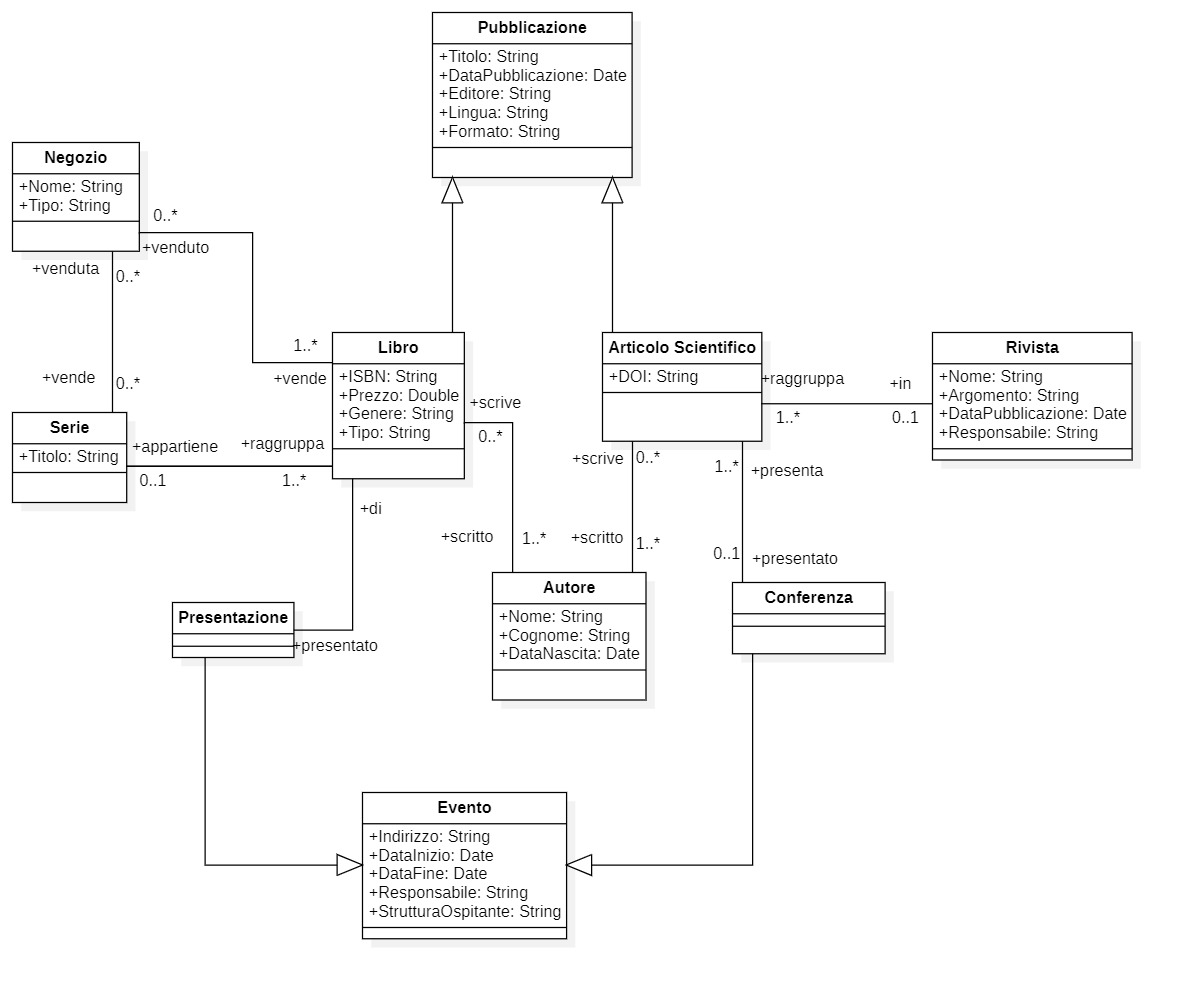
\includegraphics[scale=0.3]{Immagini/UML_v1_0.png}
        
    \section{Analisi della ristrutturazione del Class Diagram}
        In questa fase verranno effettueremo delle modifiche che renderanno il Class Diagram
        più adatto a una traduzione al modello logico \textcolor{red}{(magari scriviamo meglio sta parte)}
        \subsection{Analisi delle ridondanze}
        \textcolor{red}{(non saprei)}
        \subsection{Analisi degli identificativi}
        In questa fase andremo a scegliere uno o più attributi atti a identificare univocamente
        le varie entità presenti nello schema precedente, in particolare:
            \begin{enumerate}
            \item L'entità \textbf{Libro} presenta l'attributo ISBN che rappresenta una possibile chiave primaria,
                  tuttavia è stato scelto di aggiungere un attributo \textit{ID\_Libro} in modo tale da aumentare
                  la velocità di accesso agli indici.
            \item Per \textbf{Articolo scientifico} la situazione è analoga, è stato quindi aggiunto un attributo
                  \textit{ID\_Articolo}.
            \item Nel caso dell'entità \textbf{Rivista}, la quale presenta un attributo ISSN che è chiave candidata,
                  di inserire un ulteriore attributo \textit{ID\_Rivista}.
            \item Sarebbe possibile identificare un \textbf{Evento} tramite un insieme piuttosto ampio di attributi, è
                  stato quindi aggiunto un attributo \textit{ID\_Evento}
            \item \textbf{Autore}: 
            \item \textbf{Negozio}:
            \item \textbf{Serie}: 
            \end{enumerate}
        \subsection{Rimozione degli attributi multipli}
            
        \subsection{Rimozione degli attributi composti}
            
        \subsection{Partizione/Accorpamento delle associazioni}
            
        \subsection{Rimozione delle gerarchie}
    
    \section{Class Diagram ristrutturato}
    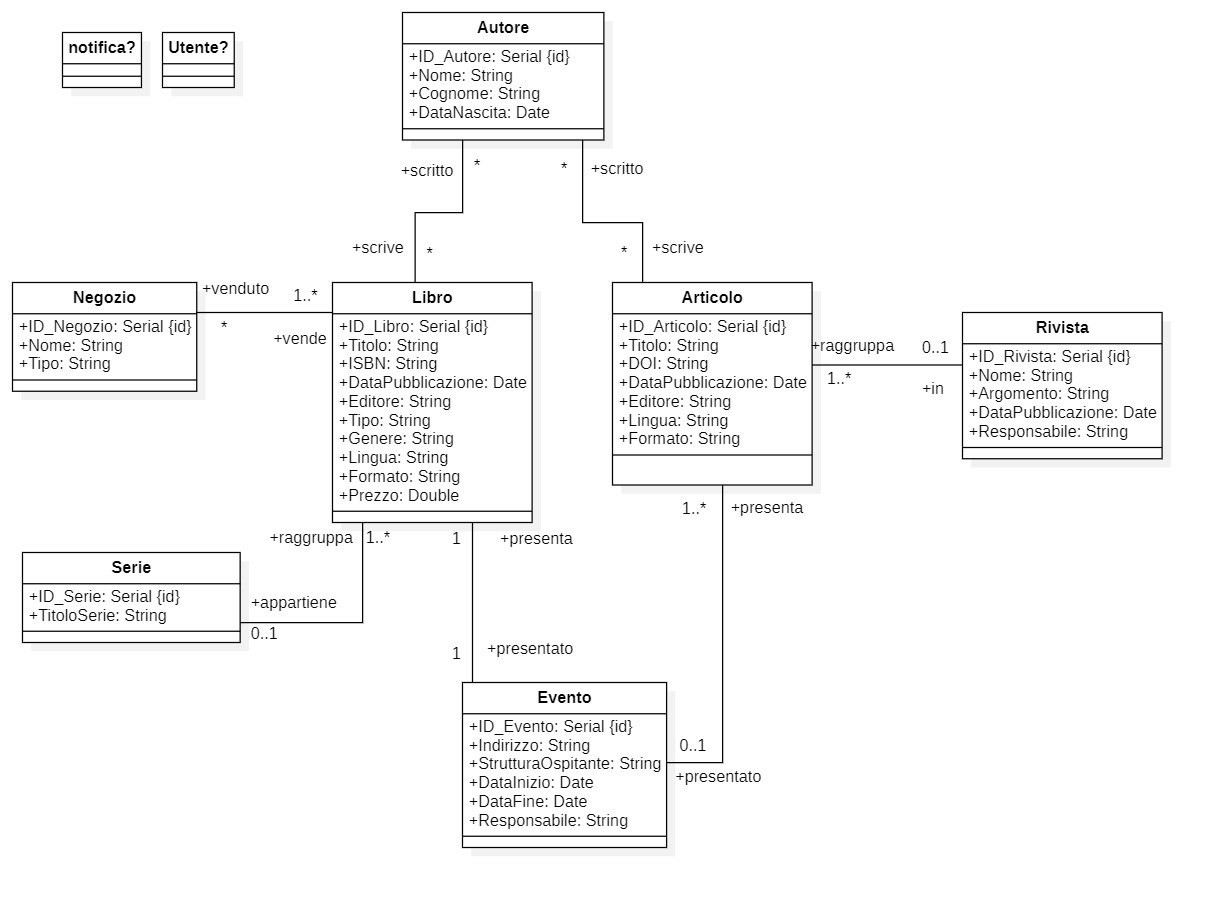
\includegraphics[scale=0.25]{Immagini/UMLris_v1_0.png}
        
    \section{Dizionario delle classi}
        
    \section{Dizionario delle associazioni}
    \chapter{Schema logico}


    \chapter{Schema Fisico}

In questo ultimo capitolo esamineremo i meccanismi necessari per la traduzione di uno schema logico 
in uno schema fisico. Andremo a definire le tabelle con i relativi attributi e tipi dei dati, le
funzioni, le procedure, i trigger e i vincoli. Con questi elementi, sar\`a possibile creare un database
relazionale con una struttura specifica che soddisfi i requisiti identificati nel Capitolo \ref{Capitolo1}.

\section{Creazione Tabelle}
\subsection{Tabella Articoli}
\begin{lstlisting}
    CREATE TABLE b.Articoli
    ID_Articolo       SERIAL,
    Titolo            VARCHAR(128),
    DOI               VARCHAR(128),
    DataPubblicazione DATE,
    Disciplina        VARCHAR(128),
    Editore           VARCHAR(128),
    Lingua            VARCHAR(128),
    Formato           VARCHAR(128),

    CONSTRAINT PK_Articoli PRIMARY KEY (ID_Articolo),
    CONSTRAINT UK_Articolo UNIQUE (DOI);
\end{lstlisting}
\subsection{Tabella Autore}
\begin{lstlisting}
    CREATE TABLE b.Autore
    ID_Autore SERIAL,
    Nome      VARCHAR(128),
    Cognome   VARCHAR(128),

    CONSTRAINT PK_Autore PRIMARY KEY (ID_Autore);
\end{lstlisting}
\subsection{Tabella AutoreArticolo}
\begin{lstlisting}
    CREATE TABLE b.AutoreArticolo
    ID_Autore   SERIAL,
    ID_Articolo SERIAL,

    CONSTRAINT PK_AutoreArticolo PRIMARY KEY (ID_Autore, ID_Articolo),
    CONSTRAINT FK_AutoreArticolo_Autore FOREIGN KEY (ID_Autore) REFERENCES b.Autore (ID_Autore) ON DELETE CASCADE,
    CONSTRAINT FK_AutoreArticolo_Articoli FOREIGN KEY (ID_Articolo) REFERENCES b.Articoli (ID_Articolo) ON DELETE CASCADE;
\end{lstlisting}

\subsection{Tabella Riviste}
\begin{lstlisting}
    CREATE TABLE b.Riviste
    ID_Rivista        SERIAL,
    ISSN              VARCHAR(128),
    Nome              VARCHAR(128),
    Argomento         VARCHAR(128),
    Responsabile      VARCHAR(128),
    Prezzo            FLOAT,

    CONSTRAINT PK_Riviste PRIMARY KEY (ID_Rivista);
\end{lstlisting}

\subsection{Tabella ArticoliInRiviste}
\begin{lstlisting}
CREATE TABLE b.ArticoliInRiviste
    ID_Articolo SERIAL,
    ID_Rivista  SERIAL,

    CONSTRAINT PK_ArticoliInRiviste PRIMARY KEY (ID_Articolo, ID_Rivista),
    CONSTRAINT FK_ArticoliInRiviste_Articolo FOREIGN KEY (ID_Articolo) REFERENCES b.Articoli (ID_Articolo) ON DELETE CASCADE,
    CONSTRAINT FK_ArticoliInRiviste_Rivista FOREIGN KEY (ID_Rivista) REFERENCES b.Riviste (ID_Rivista) ON DELETE CASCADE
\end{lstlisting}

\newpage

\subsection{Tabella Evento}
\begin{lstlisting}
    ID_Evento          SERIAL,
    Nome               VARCHAR(128),
    Indirizzo          VARCHAR(128),
    StrutturaOspitante VARCHAR(128),
    DataInizio         DATE,
    DataFine           DATE,
    Responsabile       VARCHAR(128),

    CONSTRAINT PK_Evento PRIMARY KEY (ID_Evento),
    CONSTRAINT CK_Date CHECK (DataInizio <= DataFine),
    CONSTRAINT UK_Evento UNIQUE CONSTRAINT UK_Evento UNIQUE (Nome, Indirizzo, DataInizio)
\end{lstlisting}

\subsection{Tabella Conferenza}
\begin{lstlisting}
    CREATE TABLE b.Conferenza
    ID_Articolo SERIAL,
    ID_Evento   SERIAL,

    CONSTRAINT PK_Conferenza PRIMARY KEY (ID_Articolo, ID_Evento),
    CONSTRAINT FK_Conferenza_Articolo FOREIGN KEY (ID_Articolo) REFERENCES b.Articoli (ID_Articolo) ON DELETE CASCADE,
    CONSTRAINT FK_Conferenza_Evento FOREIGN KEY (ID_Evento) REFERENCES b.Evento (ID_Evento) ON DELETE CASCADE;
\end{lstlisting}

\subsection{Tabella Libri}
\begin{lstlisting}
    CREATE TABLE b.Libri
    ID_Libro          SERIAL,
    Titolo            VARCHAR(128),
    ISBN              VARCHAR(128),
    DataPubblicazione DATE,
    Editore           VARCHAR(128),
    Genere            VARCHAR(128),
    Lingua            VARCHAR(128),
    Formato           VARCHAR(128),
    Prezzo            FLOAT,

    CONSTRAINT PK_Libri PRIMARY KEY (ID_Libro),
    CONSTRAINT UK_Libro UNIQUE (ISBN),
    CONSTRAINT CK_Libri CHECK (Prezzo > 0),
    CONSTRAINT CK_Titolo (Titolo IS NOT NULL);
\end{lstlisting}

\subsection{Tabella AutoreLibro}
\begin{lstlisting}
    CREATE TABLE b.AutoreLibro
    ID_Autore SERIAL,
    ID_Libro  SERIAL,

    CONSTRAINT PK_AutoreLibro PRIMARY KEY (ID_Autore, ID_Libro),
    CONSTRAINT FK_AutoreLibro_Autore FOREIGN KEY (ID_Autore) REFERENCES b.Autore (ID_Autore) ON DELETE CASCADE,
    CONSTRAINT FK_AutoreLibro_Libro FOREIGN KEY (ID_Libro) REFERENCES b.Libri (ID_Libro) ON DELETE CASCADE;
\end{lstlisting}

\subsection{Tabella Presentazione}
\begin{lstlisting}
    CREATE TABLE b.Presentazione
    ID_Evento SERIAL,
    ID_Libro  SERIAL,

    CONSTRAINT PK_Presentazione PRIMARY KEY (ID_Evento, ID_Libro),
    CONSTRAINT FK_Presentazione_Evento FOREIGN KEY (ID_Evento) REFERENCES b.Evento (ID_Evento) ON DELETE CASCADE,
    CONSTRAINT FK_Presentazione_Libro FOREIGN KEY (ID_Libro) REFERENCES b.Libri (ID_Libro) ON DELETE CASCADE;
\end{lstlisting}

\subsection{Tabella Serie}
\begin{lstlisting}
    CREATE TABLE b.Serie
    ID_Serie SERIAL,
    ISSN     VARCHAR(128),
    Nome     VARCHAR(128),

    CONSTRAINT PK_Serie PRIMARY KEY (ID_Serie),
    CONSTRAINT UK_Serie UNIQUE (ISSN);
\end{lstlisting}

\newpage

\subsection{Tabella LibriInSerie}
\begin{lstlisting}
    CREATE TABLE b.LibriInSerie
    ID_Serie INTEGER,
    ID_Libro INTEGER,

    CONSTRAINT PK_LibriInSerie PRIMARY KEY (ID_Serie, ID_Libro),
    CONSTRAINT FK_Libri_Serie FOREIGN KEY (ID_Serie) REFERENCES b.Serie (ID_Serie) ON DELETE CASCADE,
    CONSTRAINT FK_Serie_Libri FOREIGN KEY (ID_Libro) REFERENCES b.Libri (ID_Libro) ON DELETE CASCADE;
\end{lstlisting}

\subsection{Tabella Negozio}
\begin{lstlisting}
    CREATE TABLE b.Negozio
    ID_Negozio SERIAL,
    Nome       VARCHAR(128),
    Tipo       VARCHAR(128),

    CONSTRAINT PK_Negozio PRIMARY KEY (ID_Negozio);
\end{lstlisting}

\subsection{Tabella Stock}
\begin{lstlisting}
    CREATE TABLE b.Negozio
    ID_Negozio SERIAL,
    Nome       VARCHAR(128),
    Tipo       VARCHAR(128),

    CONSTRAINT PK_Negozio PRIMARY KEY (ID_Negozio);
\end{lstlisting}

\subsection{Tabella Utente}
\begin{lstlisting}
    CREATE TABLE b.Utente
    ID_Utente SERIAL,
    Username  VARCHAR(128),
    Password  VARCHAR(128),

    CONSTRAINT PK_Utente PRIMARY KEY (ID_Utente),
    CONSTRAINT UK_Utente UNIQUE (Username);
\end{lstlisting}

\subsubsection{TipoUtente}
\begin{lstlisting}
    CREATE TYPE b.TipoUtente AS ENUM ('0', '1', '2');
\end{lstlisting}

\newpage

\subsection{Tabella Richiesta}
\begin{lstlisting}
    CREATE TABLE b.Richiesta
    ID_Utente     SERIAL,
    ID_Serie      SERIAL,

    CONSTRAINT PK_Richiesta PRIMARY KEY (ID_Utente, ID_Serie),
    CONSTRAINT FK_Richiesta_Utente FOREIGN KEY (ID_Utente) REFERENCES b.Utente (ID_Utente) ON DELETE CASCADE,
    CONSTRAINT FK_Richiesta_Serie FOREIGN KEY (ID_Serie) REFERENCES b.Serie (ID_Serie) ON DELETE CASCADE;
\end{lstlisting}

\subsection{Tabella Jolly}
La tabella Jolly \`e una tabella che contiene un solo attributo di tipo text, che permette di
inserire una stringa di lunghezza arbitraria negli inserimenti tramite view, se necessario.
\begin{lstlisting}
    CREATE TABLE b.Jolly
    Text TEXT;
\end{lstlisting}

\section{Creazione Funzioni}

\subsection{Procedura inserimento Autori}
\begin{lstlisting}
CREATE OR REPLACE PROCEDURE b.insAutori(stringAutori text, idRisorsa INTEGER, tipoRisorsa INTEGER) AS
$$
DECLARE
    autori        text[]  = string_to_array(stringAutori, ' ');
    numAutori     INTEGER = array_length(autori, 1);
    autoreNome    b.autore.nome%TYPE;
    autoreCognome b.autore.cognome%TYPE;
    idAutore      b.autore.id_autore%TYPE;
    BEGIN
    FOR i IN 1..numAutori
        LOOP
            autoreNome = split_part(autori[i], '_', 1);
            autoreCognome = split_part(autori[i], '_', 2);
            IF NOT EXISTS(SELECT * FROM b.autore WHERE nome = autoreNome AND cognome = autoreCognome) THEN
                RAISE NOTICE 'Autore non presente, verr\`a inserito';
                INSERT INTO b.autore (nome, cognome) VALUES (autoreNome, autoreCognome);
            END IF;
            idAutore = (SELECT id_autore FROM b.autore WHERE nome = autoreNome AND cognome = autoreCognome);
            IF(tipoRisorsa = 1) THEN
                INSERT INTO b.autorelibro (id_autore, id_libro) VALUES (idAutore, idRisorsa);
            ELSEIF(tipoRisorsa = 0) THEN
                INSERT INTO b.autorearticolo (id_autore, id_articolo) VALUES (idAutore, idRisorsa);
            END IF;
        END LOOP;
END
$$ LANGUAGE plpgsql;
\end{lstlisting}

\subsection{Funzione Disponibilit\`a Libro}
\begin{lstlisting}
CREATE OR REPLACE FUNCTION b.getDisponibilitaLibro(inputLibro b.libri.id_libro%TYPE) RETURNS boolean AS
$$
DECLARE
BEGIN
    IF EXISTS(SELECT * FROM b.stock s WHERE s.id_libro = inputLibro) THEN
        return true;
    ELSE
        return false;
    END IF;
END;
$$ language plpgsql;
\end{lstlisting}

\subsection{Funzione Disponibilit\`a Serie}
\begin{lstlisting}
CREATE OR REPLACE FUNCTION b.getDisponibilitaSerie(inputSerie b.Serie.id_serie%TYPE) RETURNS boolean AS
$$
DECLARE
    scorrilibri b.libri.id_libro%TYPE;
    cursoreLibri CURSOR FOR (SELECT id_libro
                             FROM b.libriinserie
                             WHERE id_serie = inputSerie);
BEGIN
    OPEN cursorelibri;
    LOOP
        FETCH cursoreLibri INTO scorrilibri;
        EXIT WHEN NOT FOUND;
        IF NOT b.getDisponibilitaLibro(scorrilibri) THEN
            CLOSE cursoreLibri;
            return false;
        END IF;
    END LOOP;
    CLOSE cursoreLibri;
    return true;
END;
$$ language plpgsql;
\end{lstlisting}

\section{Trigger Gestione Articoli}
Per gestire l'inserimento degli articoli, vengono utilizzati due trigger,
\texttt{trig\_ArticoliRivista} e \texttt{trig\_ArticoliConferenze}, che agiscono sulle view
\texttt{ins\_ArticoliRivista} e \texttt{ins\_ArticoliConferenza}. Questi trigger verificano che la rivista 
o la conferenza non siano gi\`a presenti nel database e, in caso contrario, provvedono all'inserimento. Successivamente, 
l'articolo viene inserito e la tabella di relazione tra articoli e riviste o conferenze viene aggiornata. 
Inoltre, viene richiamata la procedura \texttt{insAutori}, che verifica se gli autori sono gi\`a presenti 
nel database e, in caso contrario, procede con il loro inserimento, seguendo l'aggiornamento della tabella 
di relazione tra articoli ed autori.
Per rimuovere gli articoli dal database, viene utilizzato il trigger \texttt{trig\_RimozioneArticoli}, che 
agisce sulla tabella \texttt{Articoli} in \texttt{BEFORE DELETE}. Questo trigger verifica che gli autori 
dell'articolo non abbiano scritto altro e, in caso affermativo, procede con la loro rimozione. Controlla 
inoltre che la rivista in cui potrebbe essere stato presentato l'articolo non abbia altri articoli e, in 
questo caso, provvede alla sua rimozione. La stessa cosa avviene per le conferenze.
\subsection{Inserimento Articolo e Rivista}
\begin{lstlisting}
    --View da dove viene inserito un articolo scientifico e la rivista dove \`e stato presentato
    CREATE OR REPLACE VIEW b.ins_ArticoliRivista AS
    SELECT a.doi,
           a.titolo,
           TEXT           as AutoriNome_Cognome, --'nome1 cognome1, nome2 cognome2'
           a.datapubblicazione,
           a.disciplina,
           a.editore,
           a.lingua,
           a.formato,
           r.nome         as nomeRivista,
           r.issn         as issnRivista,
           r.argomento    as argomentoRivista,
           r.responsabile as responsabileRivista,
           r.prezzo       as prezzoRivista
    FROM b.Articoli a,
         b.jolly,
         b.riviste r;
    
    --Funzione del trigger
    CREATE OR REPLACE FUNCTION b.ftrig_ArticoliRivista() RETURNS trigger AS
    $$
    DECLARE
        idRivista  b.riviste.id_rivista%TYPE;
        idArticolo INTEGER;
    BEGIN
        --Controllo che l'articolo non sia gi\`a presente nel DataBase
        IF EXISTS(SELECT * FROM b.articoli WHERE doi = NEW.doi) THEN
            RAISE NOTICE 'Articolo gi\`a presente, non verr\`a inserito';
        ELSE
            --Controllo che la rivista non sia gi\`a presente nel DataBase in tal caso la inserisco
            IF NOT EXISTS(SELECT * FROM b.riviste WHERE issn = NEW.issnRivista) THEN
                RAISE NOTICE 'Rivista non presente, verr\`a inserita';
                INSERT INTO b.riviste (nome, issn, argomento, datapubblicazione, responsabile, prezzo)
                VALUES (NEW.nomeRivista, NEW.issnRivista, NEW.argomentoRivista, NEW.datapubblicazione, NEW.responsabileRivista, NEW.prezzoRivista);
                --Controllo che la rivista presente nel database abbia la stessa data di pubblicazione
            ELSEIF NOT EXISTS(SELECT datapubblicazione
                              FROM b.riviste
                              WHERE issn = NEW.issnRivista
                                AND datapubblicazione = NEW.datapubblicazione) THEN
                RAISE NOTICE 'Rivista gi\`a presente ma con data di pubblicazione diversa, l''articolo non verr\`a inserito';
                RETURN NEW;
            END IF;
            --Inserisco l'articolo
            INSERT INTO b.articoli (doi, titolo, datapubblicazione, disciplina, editore, lingua, formato)
            VALUES (NEW.doi, NEW.titolo, NEW.datapubblicazione, NEW.disciplina, NEW.editore, NEW.lingua, NEW.formato);
    
            --Recupero l'id dell'articolo appena inserito
            idArticolo = (SELECT id_articolo FROM b.articoli WHERE doi = NEW.doi);
    
            --Inserisco gli autori richiamando la procedura insAutori
            CALL b.insAutori(NEW.AutoriNome_Cognome, idArticolo, 0);
    
            --Inserisco l'articolo nella rivista
            idRivista = (SELECT id_rivista FROM b.riviste WHERE issn = NEW.issnRivista);
            INSERT INTO b.articoliInRiviste (id_articolo, id_rivista) VALUES (idArticolo, idRivista);
        END IF;
        RETURN NEW;
    END;
    $$ LANGUAGE plpgsql;
    
    --Trigger per l'inserimento di un articolo scientifico e la rivista dove \`e stato presentato
    CREATE OR REPLACE TRIGGER trig_ArticoliRivista
        INSTEAD OF INSERT
        ON b.ins_ArticoliRivista
        FOR EACH ROW
    EXECUTE FUNCTION b.ftrig_ArticoliRivista();
\end{lstlisting}

\subsection{Inserimento Articolo e Conferenza}
\begin{lstlisting}
--View da dove viene inserito un articolo scientifico e la conferenza dove \`e stato presentato
CREATE OR REPLACE VIEW b.ins_articoliConferenze AS
SELECT a.doi,
       a.titolo,
       TEXT                 as AutoriNome_Cognome, --'nome1 cognome1 nome2 cognome2'
       a.datapubblicazione,
       a.disciplina,
       a.editore,
       a.lingua,
       a.formato,
       e.nome               as nomeConferenza,
       e.indirizzo          as indirizzoConferenza,
       e.strutturaospitante as strutturaospitanteConferenza,
       e.datainizio         as datainizioConferenza,
       e.datafine           as datafineConferenza,
       e.responsabile       as responsabileConferenza
FROM b.Articoli a,
     b.jolly,
     b.evento e;

--Funzione del trigger
CREATE OR REPLACE FUNCTION b.ftrig_ArticoliConferenze() RETURNS TRIGGER AS
$$
DECLARE
    idArticolo   INTEGER;
    idConferenza b.evento.id_evento%TYPE;
BEGIN
    --Controllo che l'articolo non sia gi\`a presente nel DataBase
    IF EXISTS(SELECT * FROM b.articoli WHERE doi = NEW.doi) THEN
        RAISE NOTICE 'Articolo gi\`a presente, non verr\`a inserito';
        --Controllo se la data di pubblicazione dell'articolo \`e compresa tra la data di inizio e la data di fine della conferenza
    ELSEIF (NEW.datapubblicazione < NEW.datainizioConferenza OR NEW.datapubblicazione > NEW.datafineConferenza) THEN
        RAISE NOTICE 'La data di pubblicazione dell''articolo non \`e compresa tra la data di inizio e la data di fine della conferenza, l''articolo non verr\`a inserito';
    ELSE
        --Controllo che la conferenza non sia gi\`a presente nel DataBase in tal caso la inserisco
        IF NOT EXISTS(SELECT *
                      FROM b.evento
                      WHERE nome = NEW.nomeConferenza
                        AND indirizzo = NEW.indirizzoConferenza
                        AND datainizio = NEW.dataInizioConferenza) THEN
            RAISE NOTICE 'Conferenza non presente, verr\`a inserita';
            INSERT INTO b.evento (nome, indirizzo, strutturaospitante, datainizio, datafine, responsabile)
            VALUES (NEW.nomeConferenza, NEW.indirizzoConferenza, NEW.strutturaospitanteConferenza,
                    NEW.datainizioConferenza, NEW.datafineConferenza, NEW.responsabileConferenza);
        END IF;
        --Inserisco l'articolo
        INSERT INTO b.articoli (doi, titolo, datapubblicazione, disciplina, editore, lingua, formato)
        VALUES (NEW.doi, NEW.titolo, NEW.datapubblicazione, NEW.disciplina, NEW.editore, NEW.lingua, NEW.formato);

        --Recupero l'id dell'articolo appena inserito
        idArticolo = (SELECT id_articolo FROM b.articoli WHERE doi = NEW.doi);

        --Inserisco gli autori richiamando la procedura insAutori
        CALL b.insAutori(NEW.AutoriNome_Cognome, idArticolo, 0);

        --Inserisco l'articolo nella conferenza
        idConferenza = (SELECT id_evento
                        FROM b.evento
                        WHERE nome = NEW.nomeConferenza AND indirizzo = NEW.indirizzoConferenza);
        INSERT INTO b.Conferenza (id_articolo, id_evento) VALUES (idArticolo, idConferenza);
    END IF;
    RETURN NEW;
END ;
$$ LANGUAGE plpgsql;

--Trigger per l'inserimento di un articolo scientifico e la conferenza dove \`e stato presentato
CREATE OR REPLACE TRIGGER trig_ArticoliConferenze
    INSTEAD OF INSERT
    ON b.ins_ArticoliConferenze
    FOR EACH ROW
EXECUTE FUNCTION b.ftrig_ArticoliConferenze();
\end{lstlisting}

\subsection{Rimozione Articolo}
\begin{lstlisting}
    CREATE OR REPLACE FUNCTION b.ftrig_rimozineArticoli() RETURNS trigger AS
$$
DECLARE
    idAutoreArticolo b.autore.id_autore%TYPE;
    idAutoreArticoli CURSOR FOR SELECT id_autore
                                FROM b.autorearticolo
                                WHERE id_articolo = OLD.id_articolo;
    idRivista        b.riviste.id_rivista%TYPE = (SELECT id_rivista
                                                  FROM b.articoliinriviste
                                                  WHERE id_articolo = OLD.id_articolo);
    IdConferenza     b.evento.id_evento%TYPE   = (SELECT id_evento
                                                  FROM b.conferenza
                                                  WHERE id_articolo = OLD.id_articolo);
BEGIN
    --Rimuovo gli autori se non hanno scritto altri articoli o libri
    OPEN idAutoreArticoli;
    LOOP
        FETCH idAutoreArticoli INTO idAutoreArticolo;
        EXIT WHEN NOT FOUND;
        IF NOT EXISTS(SELECT id_autore
                      FROM b.autorearticolo
                      WHERE id_autore = idAutoreArticolo
                        AND id_articolo <> OLD.id_articolo) THEN
            IF NOT EXISTS(SELECT * FROM b.autorelibro WHERE id_autore = idAutoreArticolo) THEN
                DELETE FROM b.autore WHERE id_autore = idAutoreArticolo;
            END IF;
        END IF;
    END LOOP;

    --Rimuovo la Rivista se non ha altri articoli
    IF NOT EXISTS(SELECT *
                  FROM b.articoliinriviste
                  WHERE id_articolo <> old.id_articolo
                    AND id_rivista = idRivista) THEN
        DELETE FROM b.riviste WHERE id_rivista = idRivista;
    END IF;

    --Rimuovo Conferenza se non ha altri articoli
    IF NOT EXISTS(SELECT *
                  FROM b.conferenza
                  WHERE id_articolo <> old.id_articolo
                    AND id_evento = IdConferenza) THEN
        DELETE FROM b.evento WHERE id_evento = IdConferenza;
    END IF;

    CLOSE idAutoreArticoli;
    RETURN NEW;
END;
$$ LANGUAGE plpgsql;

--Trigger per la rimozione di un articolo scientifico
CREATE TRIGGER trig_rimozioneArticoli
    BEFORE DELETE
    ON b.articoli
    FOR EACH ROW
EXECUTE PROCEDURE b.ftrig_rimozineArticoli();
\end{lstlisting}

\section{Trigger Gestione Libri}
Il trigger \texttt{trig\_Libri} agisce sulla view \texttt{ins\_Libri} per l'inserimento di un libro.
Questo trigger controlla se il libro \`e gi\`a presente nel database, e se fa parte di una serie. Se la 
serie non \`e presente nel database, la inserisce. Inoltre, riempie la tabella di relazione tra libri e serie, 
e richiama la procedura \texttt{insAutori}, che verifica che gli autori siano gi\`a presenti nel database; in 
caso negativo, li inserisce e riempie la tabella di relazione tra libri ed autori.
Per l'inserimento di una possibile presentazione di un libro si usa il trigger \texttt{trig\_presentazione}, 
che agisce sulla view \texttt{ins\_presentazione}. Tale trigger controlla che il libro sia presente nel DB, 
e se non abbia gi\`a abbia una presentazione. In tal caso, aggiunge la presentazione nella tabella \texttt{Evento}, 
riempiendo poi la tabella \texttt{Presentazione} (la tabella associativa tra \texttt{Libro} ed \texttt{Evento}).
Per la rimozione dei libri dal DB utilizziamo il trigger \texttt{trig\_rimozionelibri}, che agisce sulla tabella 
\texttt{Libri} in \texttt{BEFORE DELETE}. Questo trigger controlla che gli autori di quel libro non abbiano scritto 
altro, ed in tal caso rimuove tali autori. Controlla inoltre se la serie in cui \`e possibile che il libro sia presente 
non ha altri libri, rimuovendo la serie stessa. Infine, rimuove l'eventuale presentazione di quel libro.

\subsection{Inserimento Libro}
\begin{lstlisting}
    --View da dove viene inserito un libro
    CREATE OR REPLACE VIEW b.ins_Libri AS
    SELECT l.titolo,
           l.ISBN,
           j.TEXT as AutoriNome_Cognome, --'Nome1_Cognome1 Nome2_Cognome2'
           l.datapubblicazione,
           l.Editore,
           l.Genere,
           l.Lingua,
           l.Formato,
           l.Prezzo,
           s.nome as NOME_Serie_di_Appartenenza,
           s.ISSN as ISSN_Serie_di_Appartenenza
    FROM b.libri as l,
         b.serie as s,
         b.jolly as j;
    
    --Funzione del trigger per l'inserimento di un libro
    CREATE OR REPLACE FUNCTION b.ftrig_Libri() RETURNS TRIGGER AS
    $$
    DECLARE
        idLibro b.libri.ID_Libro%TYPE;
        idSerie b.serie.ID_Serie%TYPE;
    BEGIN
        --Controllo che il libro non sia gi\`a presente nel DataBase
        IF EXISTS(SELECT * FROM b.libri WHERE isbn = NEW.isbn) THEN
            RAISE NOTICE 'Libro gi\`a presente';
        ELSE
            --Controllo che la serie di appartenenza del libro non sia gi\`a presente nel DataBase in tal caso la inserisco
                IF NOT EXISTS(SELECT * FROM b.riviste WHERE issn = NEW.issn_serie_di_appartenenza) THEN
                RAISE NOTICE 'Serie non presente';
                IF NEW.nome_serie_di_appartenenza IS NOT NULL THEN
                    INSERT INTO b.serie(nome, issn) values (NEW.nome_serie_di_appartenenza, NEW.issn_serie_di_appartenenza);
                END IF;
                --Controllo che il formato del libro sia compatibile con la serie gi\`a presente nel DataBase
            ELSEIF NOT EXISTS(SELECT *
                              FROM (b.serie s NATURAL JOIN libriinserie ls)
                                       JOIN libri l ON ls.id_libro = l.id_libro
                              WHERE l.formato = NEW.formato) THEN
                RAISE NOTICE 'Il formato del libro non \`e compatibile con la serie, libro non inserito';
                RETURN NEW;
            END IF;
            --Inserisco il libro
            INSERT INTO b.libri (titolo, isbn, datapubblicazione, editore, genere, lingua, formato, prezzo)
            VALUES (NEW.titolo, NEW.isbn, NEW.datapubblicazione, NEW.editore, NEW.genere, NEW.lingua, NEW.formato,
                    NEW.prezzo);
            --Recupero l'id del libro appena inserito
            idLibro = (SELECT id_libro FROM b.libri WHERE isbn = NEW.isbn);
    
            --Inserisco gli autori richiamando la procedura insAutori
            CALL b.insAutori(NEW.autoriNome_cognome, idLibro, 1);
    
            --Inserisco il libro nella serie
            idSerie = (SELECT id_serie FROM b.serie WHERE issn = NEW.issn_serie_di_appartenenza);
            RAISE NOTICE 'idSerie: %', idSerie;
            IF idSerie IS NOT NULL THEN
            INSERT INTO b.libriinserie (id_libro, id_serie) VALUES (idLibro, idSerie);
            END IF;
        END IF;
        RETURN NEW;
    END
    $$ LANGUAGE plpgsql;
    
    --Trigger per l'inserimento di un libro
    CREATE OR REPLACE TRIGGER trig_Libri
        INSTEAD OF INSERT
        ON b.ins_libri
        FOR EACH ROW
    EXECUTE FUNCTION b.ftrig_Libri();
\end{lstlisting}

\subsection{Inserimento Presentazione di un libro}
\begin{lstlisting}
    --View da dove viene inserito una presentazione
    CREATE OR REPLACE VIEW b.ins_presentazione AS
    SELECT l.ISBN,
           e.nome,
           e.Indirizzo,
           e.StrutturaOspitante,
           e.DataInizio,
           e.DataFine,
           e.Responsabile
    FROM b.evento as e,
         b.libri as l;
    
    --Funzione del trigger per l'inserimento di una presentazione
    CREATE OR REPLACE FUNCTION b.ftrig_presentazione()
        RETURNS trigger AS
    $$
    DECLARE
    BEGIN
        IF NOT EXISTS(SELECT * FROM b.libri WHERE isbn = NEW.ISBN) THEN --Controllo se il libri esiste
            RAISE NOTICE 'Il libri non esiste!! Presentazione non inserita';
        ELSEIF EXISTS(SELECT *
                      FROM (b.evento as e NATURAL JOIN b.presentazione as p) --Controllo se esiste gi\`a una presentazione per quel libri
                               JOIN b.libri as l ON p.id_libro = l.id_libro
                      WHERE ISBN = NEW.ISBN) THEN
            RAISE NOTICE 'Esista gi\`a una presentazione per questo libro!! Presentazione non inserita';
        ELSE --Inserisco la presentazione
            INSERT INTO b.evento (nome, indirizzo, strutturaospitante, datainizio, datafine,
                                  responsabile) --Inserisco l'¬evento
            VALUES (NEW.nome, NEW.Indirizzo, NEW.StrutturaOspitante, NEW.DataInizio, NEW.DataFine, NEW.Responsabile);
            INSERT INTO b.presentazione (id_evento, id_libro) --Inserisco la presentazione
            SELECT e.ID_evento, l.ID_libro --Trasformo l'ISBN in un ID e recupero l'ID dell'evento
            FROM b.evento e,
                 b.libri l
            WHERE l.ISBN = NEW.ISBN
              AND e.nome = NEW.nome
              AND e.indirizzo = NEW.Indirizzo
              AND e.strutturaospitante = NEW.StrutturaOspitante
              AND e.datainizio = NEW.DataInizio
              AND e.datafine = NEW.DataFine
              AND e.responsabile = NEW.Responsabile;
        END IF;
        RETURN NEW;
    END
    $$
        language plpgsql;
    
    --Trigger per l'inserimento di una presentazione
    CREATE OR REPLACE TRIGGER trig_presentazione
        INSTEAD OF INSERT
        ON b.ins_presentazione
        FOR EACH ROW
    EXECUTE FUNCTION b.ftrig_presentazione();
\end{lstlisting}

\subsection{Rimozione Libro}
\begin{lstlisting}
    CREATE OR REPLACE FUNCTION b.ftrig_rimozineLibri() RETURNS trigger AS
$$
DECLARE
    idAutoreLibro b.autore.id_autore%TYPE;
    idAutoriLibri CURSOR FOR (SELECT id_autore
                              FROM b.autorelibro
                              WHERE id_libro = OLD.id_libro);
    idEvento      b.evento.id_evento%TYPE = (SELECT id_evento
                                             FROM b.presentazione
                                             WHERE id_libro = OLD.id_libro);
    idSerie       b.serie.id_serie%TYPE   = (SELECT id_serie
                                             FROM b.libriinserie
                                             WHERE id_libro = OLD.id_libro);
BEGIN
    --Rimuovo gli autori se non hanno scritto altri articoli o libri
    OPEN idAutoriLibri;
    LOOP
        FETCH idAutoriLibri INTO idAutoreLibro;
        EXIT WHEN NOT FOUND;
        IF NOT EXISTS(SELECT * FROM b.autorelibro WHERE id_autore = idAutoreLibro AND id_libro <> OLD.id_libro) THEN
            IF NOT EXISTS(SELECT * FROM b.autorearticolo WHERE id_autore = idAutoreLibro) THEN
                DELETE FROM b.autore WHERE id_autore = idAutoreLibro;
            END IF;
        END IF;
    END LOOP;

    --Rimuovo la presentazione del libro
    DELETE FROM b.evento WHERE id_evento = idEvento;

    --Rimuovo la serie se non ha altri libri
    IF NOT EXISTS(SELECT * FROM b.libriinserie WHERE id_serie = idSerie AND id_libro <> OLD.id_libro) THEN
        DELETE FROM b.serie WHERE id_serie = idSerie;
    END IF;

    CLOSE idAutoriLibri;
    RETURN NEW;
END;
$$ LANGUAGE plpgsql;

--Trigger per la rimozione di un libro
CREATE TRIGGER trig_rimozioneLibri
    BEFORE DELETE
    ON b.libri
    FOR EACH ROW
EXECUTE PROCEDURE b.ftrig_rimozineLibri();
\end{lstlisting}

\section{Trigger Gestione Stock}
Utilizziamo il trigger \textit{trig\_stock} che agisce sulla view \textit{ins\_stock} per gestire lo stock. 
Il trigger verifica che il libro sia presente nel database, poi controlla se il libro sia gi\`a in stock in 
quel negozio ed, in tal caso, aggiorna la quantit\`a dello stock. Per rimuovere un libro dallo stock c'\`e 
il trigger \textit{trig\_RimozioneDaStock} che aggiorna la quantit\`a del libro in stock, e se questa diventa 
zero elimina la tupla riferita a quel libro dalla tabella stock.
\begin{lstlisting}
    --View da dove inserisco i dati per aggiungere un libro allo stock
    CREATE VIEW b.ins_stock AS
    SELECT id_negozio,
           isbn,
           quantita
    FROM b.libri,
         b.stock;
    
    --Funzione del trigger per lo stock di un negozio
    CREATE OR REPLACE FUNCTION b.ftrig_stock() RETURNS TRIGGER AS
    $$
    DECLARE
        idLibro b.libri.id_libro%TYPE = (SELECT id_libro
                                         FROM b.libri
                                         WHERE isbn = NEW.isbn);
    BEGIN
        --Controllo se il libro \`e presente nel database
        IF NOT EXISTS(SELECT * FROM b.libri WHERE isbn = NEW.isbn) THEN
            RAISE NOTICE 'Libro non presente, inserimento non possibile';
            --Controllo se il negozio \`e presente nel database
        ELSEIF NOT EXISTS(SELECT * FROM b.negozio WHERE id_negozio = NEW.id_negozio) THEN
            RAISE NOTICE 'Negozio non presente, inserimento non possibile';
        ELSE
            --Controllo se il libro non \`e presente nello stock del negozio ed in tal caso lo inserisco
            IF NOT EXISTS(SELECT * FROM b.stock WHERE id_negozio = NEW.id_negozio AND id_libro = idLibro) THEN
                INSERT INTO b.stock (id_negozio, id_libro, quantita) VALUES (NEW.id_negozio, idLibro, NEW.quantita);
                --Altrimenti aggiorno la quantit\`a del libro nello stock del negozio
            ELSE
                UPDATE b.stock
                SET quantita = quantita + NEW.quantita
                WHERE id_negozio = NEW.id_negozio AND id_libro = idLibro;
            END IF;
        END IF;
        RETURN NEW;
    END;
    $$ language plpgsql;
    
    CREATE OR REPLACE TRIGGER trig_Stock
        INSTEAD OF INSERT
        ON b.ins_stock
        FOR EACH ROW
    EXECUTE FUNCTION b.ftrig_stock();
    
    --Funzione del trigger per l'aggiornamento dello stock di un negozio
    CREATE OR REPLACE FUNCTION b.ftrig_RimozioneDaStock() RETURNS trigger AS
    $$
    BEGIN
        --Controllo se la quantit\`a \`e 0 e in tal caso rimuovo il libro dallo stock
        if (NEW.quantita = 0) then
            DELETE FROM b.stock WHERE id_libro = OLD.id_libro;
        end if;
    END;
    $$ language plpgsql;
    
    --Trigger per l'aggiornamento dello stock di un negozio
    CREATE TRIGGER trig_RimozioneDaStock
        AFTER UPDATE OF quantita
        ON b.stock
        FOR EACH ROW
    EXECUTE FUNCTION b.ftrig_RimozioneDaStock();
\end{lstlisting}

\section{Gestione Notifiche}
L'utente pu\`o richiedere la disponibilit\`a di una serie, riempiendo la tabella \textit{richieste}. Qualora 
l'utente debba essere notificato, si utilizza la view \textit{notifiche}.

\subsection{View Notifiche}
\begin{lstlisting}
    CREATE VIEW b.notifiche AS
    SELECT *, b.getDisponibilitaSerie(id_serie) AS disponibilita
    FROM b.serie NATURAL JOIN b.richiesta
    WHERE b.getDisponibilitaSerie(id_serie) IS true;
\end{lstlisting}


\end{sloppypar}
\end{document}